\chapter{Evolución histórica}\label{AneC}

Hace 40 años las primeras tarjetas de video, ni siquiera soportaban el despliegue de gráfico/video, sólo texto, donde cada entrada permitía guardar la información para un carácter.
Ya en el primer lustro de los 80s aparecen arquitecturas como \texttt{Hercules}, pensadas en términos de píxeles. En estos casos la capacidad de memoria estaba puramente relacionada con lo que se iba a desplegar en pantalla. Poco después, aparece por ejemplo la tarjeta CGA, que permitiría almacenar colores, ahora no solo se tendrían píxeles monocromáticos sino que se tendría la posibilidad de variar cada píxel hasta 16 colores diferentes.
% Dada la baja cantidad de memoria 16kb, se podian obtener disitntas resoluciones con distinta 
Hasta la década de los 90s las tarjetas fueron mejorando en capacidad de resolución, enfocadas únicamente en el despliegue de video, recibiendo de la CPU el arreglo de píxeles que debía desplegar, sin la necesidad de realizar algún tipo de procesamiento. Durante los 90s comienzan a aparecer las primeras tarjetas, no solo enfocadas en guardar y mostrar los datos preprocesados por la CPU, sino capaces de realizar cálculos asociados a esos gráficos que se querían desplegar. Particularmente, la capacidad de reproducir efectos 2D/3D. Notar que, típicamente se deben desplegar imágenes que son proyecciones de escenas tridimensionales en una pantalla bidimensional, introduciendo el concepto de \textit{pipeline gráfico}. Una secuencia ordenada de pasos, que generalmente tienen el objetivo de proyectar estas escenas en tres dimensiones, al plano. En la Figura~\ref{fig:pipeline-example} se puede ver un ejemplo de las principales etapas del \textit{pipeline gráfico}.

\begin{figure}
    \centering
    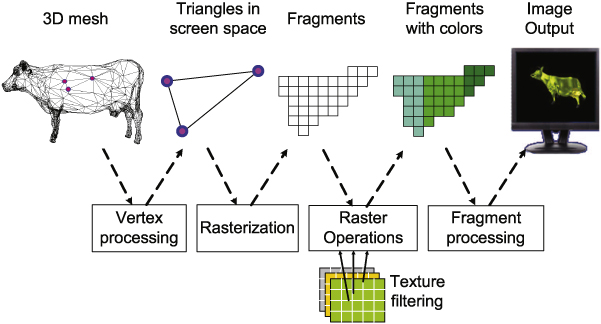
\includegraphics[width=\textwidth]{imagenes/chapter2/pipeline-example.jpg}
    \caption{Ejemplo simplificado de \textit{pipeline gráfico} para obtener una proyección bidimensional de un cuerpo en tres dimensiones. Extraído de \cite{pipeline-example}.}
    \label{fig:pipeline-example}
\end{figure}
Posteriormente, y en forma paulatina, las tarjetas gráficas fueron agregando el procesamiento de más etapas del pipeline, con el objetivo de alivianar el trabajo de la  CPU. Pasando así a resolver la pesada tarea de proyección de escenas, por ejemplo tridimensionales, al plano, tarea que antes realizaba la CPU para luego enviarla a la tarjeta para que esta la mostrara.

\deposito{
\texttt{NVIDIA} con la 256 presenta la primer GPU (Graphic Processing Unit), primer tarjeta gráfica para ``usuarios'', que implementa el pipeline gráfico completo.

% El pipeline permite procesar un flujo de datos a través de varias etapas ejecutadas secuencialmente por diferentes unidades, donde la entrada de una etapa es la salida de la anterior.

Arquitectura unificada, permitiendo que las unidades de cómputo funcionen como pixel shaders y vertex shaders, obeteniendo un unified shaders. Con esto, surge la idea del cómputo del propósito general. Por qué limitarse a procesar solo píxeles y vértices, pudiendo dedicar tal poder de cómputo a la resolución de otros problemas existentes. 

En los últimos años ha habido una explosión en la utilización de las GPUs para el cómputo de problemas de propósito general. Motivado por la pujante industria de los videojuegos y con el objetivo de resolver muchos de los problemas de la computación científica como la inteligencia artificial (redes neuronales).
Este crecimiento, está basado principalmente en los siguientes puntos:
\begin{itemize}
    \item La arquitectura de las GPUs es intrínsecamente paralela, en contraste con como fueron realizadas y concebidas las CPUs, pensadas para resolver problemas de forma secuencial (si bien en la actualidad logran trabajar de forma paralela).
    \item Como se dijo anteriormente, la industria de los videojuegos ejerce una fuerte presión a los fabricantes de tarjetas gráficas para aumentar las capacidades de procesamiento gráfico para que los juegos sean más realistas, más rápidos y con mejores resoluciones.
    \item Surgen lenguajes de programación de propósito general para GPUs, lenguajes que de manera relativamente sencilla, permitirían mapear problemas de propósito general a la arquitectura de la GPU.
\end{itemize}
}

Las GPUs en los inicios de los años 2000 no soportaban precisiones mayores a 8 bits, capaces para representar 256 colores. Posteriormente se pasó a 16 bits, permitiendo moverse entre $2^{16}$ valores, que para colores es más que suficiente. Más general aún, aumentaron otra vez el ancho con el cual se podía trabajar, pasando a trabajar con 32 bits, soportando así números en punto flotante simple precisión.

De todos modos, en principio, el avance del hardware no se vio acompañado por un avance de software para el manejo de esta arquitectura.
Inicialmente la programación de las GPUs se realizaba a través de llamados a servicios de interrupción de la BIOS, camino poco práctico, que llevaba a cometer muchos errores, además de complicar la tarea de depuración, bugs.
Posteriormente, se comenzaron a desarrollar los \texttt{shaders} en el lenguaje ensamblador con el cual se los podía programar, pero este conjunto instrucciones era específico de cada shader, que podía cambiar de generación a generación, generando grandes problemas para la programación sobre estos dispositivos.
Otra opción para programarlas, era utilizar las \texttt{APIs} gráficas como \texttt{OpenGL} y \texttt{DirectX}, pero para computación de propósito general era necesario mapear el problema en términos de triángulos, sombreados, etc y de alguna forma expresar el problema en términos de  otros conceptos.

Dados estos problemas, se comienza a desarrollar lenguajes de programación de más alto nivel, capaces de programar cada GPU existente. Sin embargo, cada lenguaje seguía siendo muy dependiente de cada arquitectura y fabricante, seguían sin presentar los suficientes niveles de abstracción.
Entonces, en el año 2007 \texttt{NVIDIA} propone CUDA (Compute Unified Device Architecture), lenguaje que permitió abstraerse en gran medida de las arquitecturas subyacentes, siendo un importante avance para la computación de propósito general en este tipo de dispositivos, que se mantiene al día de hoy.

